% ----------------------
  \chapter{Marco Teórico} 
% ----------------------
\label{C:antecedentes}
Durante el presente capítulo se desarrollará un repaso sobre los principales conceptos relacionados al proyecto, con el fin de poder consolidar una base teórica esencial para entender el mismo.
\section{Redes Neuronales}
\begin{figure}[H]
    \centering
    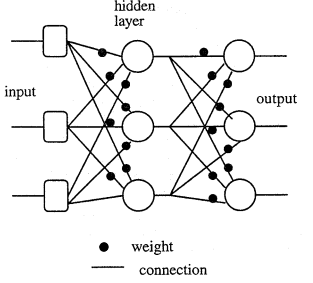
\includegraphics[width=0.5\textwidth]{imagenes/marco teorico/modelo_red.png}
    \caption{Modelo de una red neuronal \cite{nallasamy}}
    \label{neural_model}
\end{figure}
\par
En la figura \ref{neural_model}, se puede ver una representación gráfica para un modelo de una red neuronal, en este caso la aplicada por los autores en \cite{nallasamy}.
\subsection{Generalidades}
\par
Las redes neuronales como la mostrada anteriormente son una representación computacional del cerebro humano, que intenta dar funcionamiento correcto a la inteligencia artificial. La idea detrás de su creación fue poder crear un algoritmo que funcione como lo haría el cerebro humano, debido a que es la computadora más potente conocida.
\par
Al intentar asimilarse al cerebro humano también copian mecanismos utilizados por el mismo, por ejemplo aprenden de la experiencia, es decir a partir de resultados generados, reciben retroalimentación y así afinan los resultados que puedan dar a futuro \cite{olabe_2008}. Inicialmente el programador debe dar a la red una lista de entradas y una de salidas esperadas dependiendo de la entrada, luego la red deberá entrenarse para poder generar resultados que sigan el patrón de los datos iniciales.
\par
La estructura de una red neuronal artificial conlleva los mismos elementos para cualquier aplicación. Cuenta con diferentes entradas que se combinan usualmente sumadas. Luego las entradas pasan por una o varias neuronas (dependiendo de la arquitectura de la red), las cuales se llaman capas ocultas, puesto que contienen una función de transferencia que procesa los datos para luego alimentar cada una de las diferentes salidas \cite{olabe_2008}.
\par
El elemento más importante de una red neuronal, es la neurona, que en programación se puede ver como un nodo de una estructura abstracta, que genera resultados. Cada entrada se conecta a la neurona por medio de un peso, el cual representa la importancia de esta entrada y luego la neurona toma las entradas multiplicadas por su peso y sumadas, para procesarlas por medio de la función de transferencia generada del proceso de entrenamiento \cite{olabe_2008}.

\subsection{Entrenamiento de la red neuronal}
Cómo se mencionó en la sección anterior, una de las características determinantes de una red neuronal es la capacidad de aprendizaje, por lo que es normal que al inicio los resultados obtenidos con ella no sean los deseados. Para arreglar este problema no se puede utilizar la red de forma inmediata, sino que debe llevar un proceso de entrenamiento, para que a la hora de utilizarla, los resultados obtenidos de las entradas dadas sean correcto o muy aproximados.
\par
El proceso de entrenamiento realiza un ajusto en los pesos que posee cada entrada conforme recibe retroalimentación de las salidas generadas. Esto se logra aplicando diferentes entradas de forma secuencial para una obtención de salidas, que luego se verifican, para asegurar que se ajusten los pesos correctamente conforme se introducen datos \cite{olabe_2008}. Existen dos tipos de entrenamientos: supervisado y no supervisado.
\subsubsection{Entrenamiento supervisado}
El programador deberá dar a los datos de entrada provistos una salida emparejada para que la red pueda comparar y ajustar los pesos. Usualmente se ajusta por medio de un cálculo de porcentaje de error, el cual debe ir disminuyendo hasta ser un valor pequeño, que pueda considerar el resultado correcto \cite{olabe_2008}.
\subsubsection{Entrenamiento no supervisado}
En el caso del entrenamiento no supervisado, no se le provee a la red un set de datos de salida deseados, por lo que no hay comparación ni cálculo del error cometido a la hora de procesar los datos. La forma de ajuste de los pesos de cada entrada se da por medio de una comparación interna de las salidas producidas, para que formen un conjunto de datos consistente \cite{olabe_2008}. 
\subsection{Creación de una red neuronal}
Las redes neuronales pueden ser creadas o aplicadas de diferentes formas. La más compleja siendo la creación directa de la red por medio de programación haciendo uso de diferentes librerías como pueden ser: TensorFlow, Microsoft Cognitive Toolkit, PyTorch, Keras, Theano, entre otras. 
\par
El proceso de creación de una red conlleva no solamente el tiempo para poder implementarla por medio de la librería, sino que también el tiempo de entrenamiento para poder finalmente utilizarla. Es importante hacer notar que usualmente el poder computacional necesario para llevar acabo esto es bastante significativo, por lo que no es siempre conveniente.
\par
La otra forma de creación de una red neuronal, está dada por medio del uso de servicios de redes neuronales que están basadas en la nube. Usualmente son provistas por terceros y permiten modificar diferentes aspectos del modelo dependiendo de la aplicación que se quiera utilizar. Es necesario llevar acabo el ajuste de la red, así como el proceso de entrenamiento para que se pueda utilizar. Algunos de los provedores de este tipo de redes más conocidos son: Nanonets, Edge Impulse, Rossum, DarwinAI y muchas otras más.

\section{OCR}
\subsection{Generalidades}
El reconocimiento óptico de caracteres, conocido por sus siglas en inglés OCR (Optical character recognition) es el proceso de análisis y conversión de letras o caracteres de algun medio u objeto a un caracter ASCII que una computadora pueda reconocer \cite{nallasamy}.
\par
El OCR es usado por muchas aplicaciones, de las cuales se incluye la transformación de cualquier cosa humanamente legible a una representación manipulable por una computadora. El proceso permite escanear de manera óptica, por medio de una entrada de video, los caracteres que se desean procesar por la computadora. La intención del proceso de OCR es permitir a las computadoras procesar automáticamente y sin intervención humana fracciones de texto e inclusive objetos que necesiten ser procesados \cite{Shah2009}.
\par
Los sistemas que implementan OCR, se componen de tres partes principales: Una cámara, software de procesamiento de OCR y una interfaz de salida. El reconocimiento de los caracteres usualmente está procesado por inteligencia artificial (usualmente una red neuronal) que conforme procesa datos nuevos aprende a reconocerlos de mejor manera \cite{Shah2009}. La idea de implementar OCR en los sistemas es evitar el error humano, aumentar la capacidad y tiempo de procesamiento además de permitir un mejor rendimiento a la hora de leer y escribir a archivos. 

\subsection{Implementación}
La implementación del OCR por medio de software se logra con diferentes librerías que combinan la visión por computador y la inteligencia artificial para el procesamiento de las imágenes. En trabajos como los vistos en \cite{nallasamy} y \cite{Shah2009} es posible apreciar como se creó un algoritmo que procese las imágenes a partir de una red neuronal. El algoritmo también debe contemplar el pre-procesamiento de las imagenes para que sean más fácilmente leídas por la red que las procesará después.
\par
Hay múltiples librerías para la implementación de OCR para diferentes lenguajes de programación, inclusive Tesseract, el cual es una librería de redes neuronales, incluye funciones que permiten la implementación de OCR.

\section{Python}
Python es un lenguaje de programación interpretado, es decir un programa intermediario entre la computadora y el usuario (llamado interprete) lee el código y lo ejecuta línea por línea. Es un lenguaje de alto nivel, que al ser creado se pensó especialmente para desarrollo rápido, sencillo, pero aún así poderoso funcional \cite{van1995python}.
\par
Python utiliza sintaxis de escritura sencillo, pensado para la fácil lectura que reduce el costo de la corrección de errores y el fácil entendimiento a la hora de leer el código \cite{van1995python}. Lo que en lenguajes de programación compilados puede tomar varias líneas de código, en Python se reduce de forma significativa. El ejemplo más básico se da a la hora de hacer un programa que imprima "Hola Mundo" en la consola de comandos, como se muestra a continuación:

\begin{lstlisting}[language=Java,frame=single,caption=Código del Hola Mundo en Java, inputencoding=latin1]
public class HolaMundo {

	public static void main(String[] args) {		
		System.out.println("Hola Mundo");
	}

}
\end{lstlisting}
\begin{lstlisting}[language=Python,frame=single,caption=Código del Hola Mundo en Python, inputencoding=latin1]
print("Hola Mundo")
\end{lstlisting}

\par
Es posible notar de los códigos anteriores que la diferencia entre la cantidad de lineas de código en Java es muy superior a la de Python, permitiendo escribir códigos más compactos y más sencillos de leer también. Esto ha hecho que Python sea un lenguaje de programación bastante popular a nivel no-comercial, permitiendo también que se expandan los proyectos que apoyan la creación de librerías para desarrollo en él.


\subsection{Librerías}
\par
Las librerías son un complemento fundamental de la programación en Python, ya que permiten importar a un código funciones previamente escritas que realizan algún algoritmo requerido a la hora de programar \cite{van1995python}.
\par
Con ellas es posible crear códigos para diferentes áreas de aplicación, como por ejemplo el análisis de datos, inteligencia artificial, desarrollo web, ciencias de datos, big data, machine learning e inclusive desarrollo de juegos. La versatilidad que proveen las librerías en conjunto con la facilidad de programación en el lenguaje Python, hacen de la experiencia de desarrollo amigable para cualquier nivel de experiencia que se tenga.

\section{Bases de datos}
Una base de datos es una forma de organizar información o datos con algún tipo de estructura que se almacenan de forma electrónica en un sistema informático. Es decir una base de datos es un conjunto estructurado de datos que representa entidades y sus interrelaciones \cite{camps_paré_2005}.
\par
Para poder controlar las bases de datos, es necesario un gestor que permita hacer un manejo correcto de las mismas. Para ello existen los sistemas de gestión de bases de datos (SGBD). Su principal función es permitir que se hagan consultas no predefinidas y complejas, es decir que la combinación de datos que se quiere extraer de una base de datos no esté predefinida en el programa que la gestiona para que sea una búsqueda válida. Además gestiona las conexiones que se ralizan a la base, por lo que debe permitir y la conexión de varios usuarios a ella \cite{camps_paré_2005}.
\par
Las consultas a la base de datos se realizan por medio de lenguaje escrito (sintaxis) equivalente a un lenguaje de programación, pero específico del tipo de base de datos y el sistema debe interpretar el tipo de acción que se desea realizar. En la figura \ref{BDflux} se puede apreciar el flujo de las consultas a una base de datos. 
\begin{figure}[H]
    \centering
    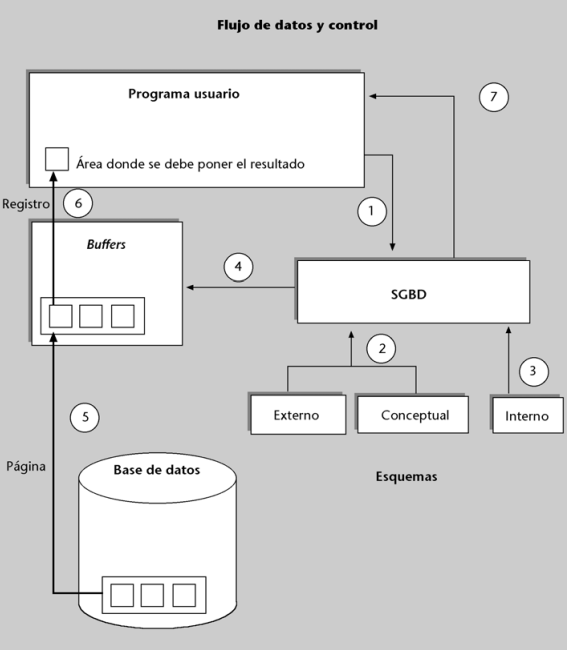
\includegraphics[width=0.4\textwidth]{imagenes/marco teorico/flujo_BD.png}
    \caption{Flujo de una consulta a una base de datos \cite{camps_paré_2005}.}
    \label{BDflux}
\end{figure}
\par
Las consultas inician de forma que se hace una llamada del programa que contacta con la base de datos al SGDB, donde se envía la operación de la consulta que se desea hacer (punto 1). El SGDB verifica que la sintaxis esté correcta y que la conexión esté autorizada a acceder (punto 2) \cite{camps_paré_2005}. 
\par
En caso de que todo esté correcto se debe asegurar que tipo de respuesta requiere la solicitud y cuál aproximación se va a tomar para responderla (punto 3). Luego se revisa si los datos se encuentran cargados en memoria por alguna solicitud previa (punto 4) y caso contrario deberá buscarla en el disco, con ayuda del sistema operativo donde se almacena la BD y cargarla al buffer (punto 5, solo en caso de que no se encuentre previamente cargada)\cite{camps_paré_2005}.
\par
El SGDB realiza operaciones necesarias para poder transportar los datos al área donde se encuentra el programa de la forma más eficiente posible (punto 6). Finalmente el SGDB retorna al programa y devuelve el control al mismo para que haga lo necesario con lo extraído de la base de datos (punto 7) \cite{camps_paré_2005}. 
\par
Con lo mencionado anteriormente es posible comprender el proceso de solicitudes a bases de datos, entiendo así el funcionamiento que se tiene detrás de muchas aplicaciones que contienen datos almacenados en bases de datos.


\subsection{Modelos de bases de datos}
\par
Las bases de datos no se presentan únicamente en un tipo de modelo, sino que a través de los años se han implementado diferentes formas de almacenar los datos dentro de una base de datos y estas se les llaman \textit{modelos de bases de datos}. Se explicará tres de los modelos que se presentan en bases de datos por su relevancia histórica o por su uso popular, siendo estas: jerárquicas, red y relacional, como se observa en la figura \ref{BDmodels}.
\begin{figure}[H]
    \centering
    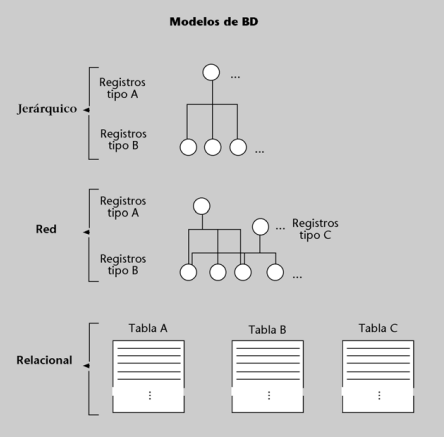
\includegraphics[width=0.5\textwidth]{imagenes/diseño/modelodb.png}
    \caption{Modelos de bases de datos \cite{camps_paré_2005}.}
    \label{BDmodels}
\end{figure}

\subsubsection{Modelo jerárquico}
\par
Fue el primer modelo de BD, surgió a principios de los sesenta. Se estructura está dada como una estructura abstracta de datos de tipo árbol, por lo que los datos están conectados por medio de nodos, que separan los niveles. Es el primer modelo mostrados en la figura \ref{BDmodels} \cite{camps_paré_2005}.

\subsubsection{Modelo de Red}
\par
La estructura de los modelos de red se asemejan a los jerárquicos, con la diferencia de que un registro puede no necesariamente ser hijo de un tipo de registro. Dando una mayor libertad a la organización de datos y su forma de almacenarlos dentro de la BD \cite{camps_paré_2005}, como se presenta en el segundo modelo de la figura \ref{BDmodels}.

\subsubsection{Modelo relacional}
\par
El tercer modelo de la figura \ref{BDmodels} es el relacional, el cual se diferencia mucho de los otros dos modelos presentados anteriormente, esto debido a que está basado en el concepto matemático de relación. Su principal elemento es la tabla, la cual es la causa del nombre que se le asigna. La tabla consta de filas y columnas, donde cada columna usualmente presente un atributo y cada fila es un registro único diferente del resto (aunque no necesariamente con diferentes columnas, a excepción de la característica principal, que es diferenciante). Es una forma intuitiva y sencilla de almacenar datos, ya que a nivel lógico tiene mucho sentido almacenarlos de esta forma, además permite la facilidad de tener más de una tabla donde puede o no alguna de sus filas tener relación con alguna fila y/o columna de otra \cite{camps_paré_2005}.

